\documentclass[12pt,letterpaper]{exam}
\usepackage[lmargin=1in,rmargin=1in,tmargin=1in,bmargin=1in]{geometry}
\usepackage{../style/exams}

% -------------------
% Course & Exam Information
% -------------------
\newcommand{\course}{MAT 307: Exam 1}
\newcommand{\term}{Spring -- 2023}
\newcommand{\examdate}{03/03/2023}
\newcommand{\timelimit}{85 Minutes}

\setbool{hideans}{true} % Student: True; Instructor: False

% -------------------
% Content
% -------------------
\begin{document}

\examtitle
\instructions{Write your name on the appropriate line on the exam cover sheet. This exam contains \numpages\ pages (including this cover page) and \numquestions\ questions. Check that you have every page of the exam. Indicate your answer for each question in the answer column in the table below. You need not indicate your answers for each question both on the cover page and in the subsequent pages. You may show as much or as little work as you would like; however, only the answers on this cover page will be graded. Be sure each answer is legible and in the correct box. Do not write in the `Points' box on this page.} 
%\scores
%\bottomline

\vfill

\begin{table}[!ht]
\hspace{-1.5cm} \resizebox{1.2\textwidth}{!}{
\begin{tabular}{|
>{\columncolor[HTML]{C0C0C0}}c |l|
>{\columncolor[HTML]{C0C0C0}}c |l|
>{\columncolor[HTML]{C0C0C0}}c |l|
>{\columncolor[HTML]{C0C0C0}}c |l|
>{\columncolor[HTML]{C0C0C0}}c |l|} \hline
% Titles
\cellcolor[HTML]{000000}{\color[HTML]{FFFFFF} \textbf{Question}} & \multicolumn{1}{c|}{\cellcolor[HTML]{000000}{\color[HTML]{FFFFFF} \textbf{Answer}}} & \cellcolor[HTML]{000000}{\color[HTML]{FFFFFF} \textbf{Question}} & \multicolumn{1}{c|}{\cellcolor[HTML]{000000}{\color[HTML]{FFFFFF} \textbf{Answer}}} & \cellcolor[HTML]{000000}{\color[HTML]{FFFFFF} \textbf{Question}} & \multicolumn{1}{c|}{\cellcolor[HTML]{000000}{\color[HTML]{FFFFFF} \textbf{Answer}}} & \cellcolor[HTML]{000000}{\color[HTML]{FFFFFF} \textbf{Question}} & \multicolumn{1}{c|}{\cellcolor[HTML]{000000}{\color[HTML]{FFFFFF} \textbf{Answer}}} & \cellcolor[HTML]{000000}{\color[HTML]{FFFFFF} \textbf{Question}} & \multicolumn{1}{c|}{\cellcolor[HTML]{000000}{\color[HTML]{FFFFFF} \textbf{Answer}}} \\ \hline
% 1 - 41
{\color[HTML]{000000} 1} &  & {\color[HTML]{000000} 11} &  & {\color[HTML]{000000} 21} &  & {\color[HTML]{000000} 31} &  & {\color[HTML]{000000} 41} &  \\ \hline
% 2 - 42
{\color[HTML]{000000} 2} &  & {\color[HTML]{000000} 12} &  & {\color[HTML]{000000} 22} &  & {\color[HTML]{000000} 32} &  & {\color[HTML]{000000} 42} &  \\ \hline
% 3 - 43
{\color[HTML]{000000} 3} &  & {\color[HTML]{000000} 13} &  & {\color[HTML]{000000} 23} &  & {\color[HTML]{000000} 33} &  & {\color[HTML]{000000} 43} &  \\ \hline
% 4 - 44
{\color[HTML]{000000} 4} &  & {\color[HTML]{000000} 14} &  & {\color[HTML]{000000} 24} &  & {\color[HTML]{000000} 34} &  & {\color[HTML]{000000} 44} &  \\ \hline
% 5 - 45
{\color[HTML]{000000} 5} &  & {\color[HTML]{000000} 15} &  & {\color[HTML]{000000} 25} &  & {\color[HTML]{000000} 35} &  & {\color[HTML]{000000} 45} &  \\ \hline
% 6 - 46
{\color[HTML]{000000} 6} &  & {\color[HTML]{000000} 16} &  & {\color[HTML]{000000} 26} &  & {\color[HTML]{000000} 36} &  & {\color[HTML]{000000} 46} &  \\ \hline
% 7 - 47
{\color[HTML]{000000} 7} &  & {\color[HTML]{000000} 17} &  & {\color[HTML]{000000} 27} &  & {\color[HTML]{000000} 37} &  & {\color[HTML]{000000} 47} &  \\ \hline
% 8 - 48 
{\color[HTML]{000000} 8} &  & {\color[HTML]{000000} 18} &  & {\color[HTML]{000000} 28} &  & {\color[HTML]{000000} 38} &  & {\color[HTML]{000000} 48} &  \\ \hline
% 9 - 49
{\color[HTML]{000000} 9} &  & {\color[HTML]{000000} 19} &  & {\color[HTML]{000000} 29} &  & {\color[HTML]{000000} 39} &  & {\color[HTML]{000000} 49} &  \\ \hline
% 10 - 50
{\color[HTML]{000000} 10} &  & {\color[HTML]{000000} 20} &  & {\color[HTML]{000000} 30} &  & {\color[HTML]{000000} 40} &  & {\color[HTML]{000000} 50} &  \\ \hline
\end{tabular}
}
\end{table}

\vspace{0.5cm}

	\begin{table}[!ht]
	\centering
	\begin{tabular}{|c|c|} \hline 
	\rowcolor[HTML]{000000} 
	{\color[HTML]{FFFFFF} Points} & {\color[HTML]{FFFFFF} Total} \\ \hline
	& 50 \\ \hline
	\end{tabular}
	\end{table}

\vspace{3cm}
\vfill

\newpage


% ---------
% Questions
% ---------
\begin{questions}

% Question 1
\question Let $A= \{ 1, 2, 3, 4, 5 \}$ and $B= \{ 3, 4, 5, 6, 7 \}$. Which of the following is $A \cup B$?
	\begin{enumerate}[A.]
	\item $\{ 4, 5 \}$
	\item $\{ 3, 4, 5 \}$
	\item $\{ 1, 2, 6, 7 \}$
	\item $\{ 1, 2, 3, 4, 5, 6, 7 \}$
	\end{enumerate}

\vfill 

% Question 2
\question How many possible unique arrangements of letters are there using the letters of the word `endless'?
	\begin{enumerate}[A.]
	\item $7$
	\item $21$
	\item $1260$
	\item $5040$
	\end{enumerate}

\vfill

% Question 3
\question If you are dealt five cards from a deck of cards, approximately what is the probability that you are dealt four kings?
	\begin{enumerate}[A.]
	\item $0.00002$
	\item $0.019$
	\item $0.077$
	\item $0.307$
	\end{enumerate}

\vfill

% Question 4
\question Alice and Bob take an exam. Alice received a 79 on her exam while Bob received a 67 on his exam. Alice's exam was normally distributed with mean 85 and standard deviation 1.5 while Bob's exam was normally distributed with mean 60 and standard deviation 5. Which of the following statements is most accurate?
	\begin{enumerate}[A.]
	\item Alice did better on her exam compared to others but Bob's score was more `unusual' compared to others. 
	\item Bob did better on his exam compared to others but Alice's score was more `unusual' compared to others. 
	\item Alice's exam score was better compared to others and her exam score was more `unusual' compared to others. 
	\item Bob's exam score was better compared to others and his exam score was more `unusual' compared to others. 
	\end{enumerate}



\newpage
\vfill


% Question 5
\question Let $A= \{ 10, 1, 5, 4, 6 \}$ and $B= \{ 3, 5, 0, -2, 6 \}$. Which of the following is the set $A - B$?
	\begin{enumerate}[A.]
	\item $\{ 1, 4, 10 \}$
	\item $\{ 7, -4, 5, 6, 0 \}$
	\item $\{ -4, 0, 5, 6, 7 \}$
	\item $\{ -2, 0, 1, 3, 4, 10 \}$
	\end{enumerate}

\vfill

% Question 6
\question Mr. Lambert has 40 students in his classroom. Of these students, 13 have been to a zoo, 15 have been to a museum, and 5 have been to both. Which of the following is the number of students that have been to neither?
	\begin{enumerate}[A.]
	\item 7
	\item 12
	\item 17
	\item 35
	\end{enumerate} 

\vfill

% Question 7
\question There are three spinners, shown below with portions of each spinner colored white or black.\par
	\[
	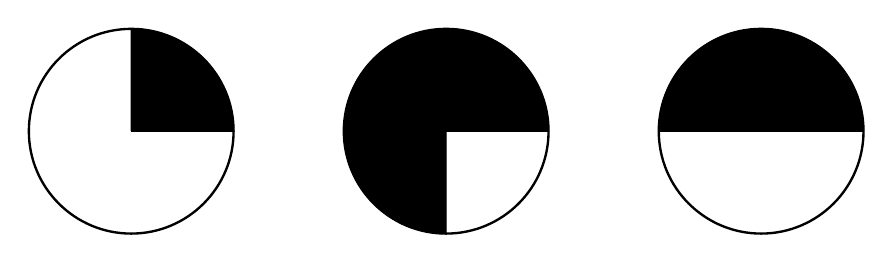
\begin{tikzpicture}
	\draw[line width=0.03cm] (0,0) circle (1.3);
	\draw[fill=black] (0,0) -- (1.3,0) arc[start angle=0, end angle=90,radius=1.3] -- (0,0);
	
	\draw[line width=0.03cm] (4,0) circle (1.3);
	\draw[fill=black] (4,0) -- (5.3,0) arc[start angle=0, end angle=270,radius=1.3] -- (4,0);

	\draw[line width=0.03cm] (8,0) circle (1.3);
	\draw[fill=black] (8,0) -- (9.3,0) arc[start angle=0, end angle=180,radius=1.3] -- (8,0);
	\end{tikzpicture} 
	\]
If you spin each of these three spinners, one after the other, what is the probability that each spinner lands in the dark shaded area?
	\begin{enumerate}[A.]
	\item $0.09375$
	\item $0.50000$
	\item $0.66667$
	\item $0.75000$
	\end{enumerate}

\vfill

% Question 8
\question Let $S$ be the set of counting numbers from 1 to 100 (including 1 and 100). Suppose you found the mean, median, IQR, and standard deviation of $S$. Which of the following statements is most accurate if you were to compute these statistics after including the number 1,200 in the set $S$?
	\begin{enumerate}[A.]
	\item The mean would change more than the median.
	\item The median would change more than the mean.
	\item The mean and median would change by the same amount.
	\item The mean would change but the median would not.
	\end{enumerate}

\vfill

% Question 9
\question Which of the following represents the region shaded in the Venn diagram below?
%	\[
%	\begin{venndiagram2sets}[tikzoptions={scale=1}]
%	\fillOnlyA
%	\end{venndiagram2sets}	
%	\]
	\begin{figure}[H]
	\centering
	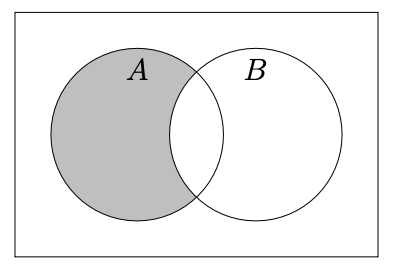
\includegraphics[width=0.30\textwidth]{venn.png}
	\end{figure}
		
	\begin{enumerate}[A.]
	\item $A$
	\item $A \cap B$
	\item $A - B$
	\item $(A \cup B) - (A \cap B)$
	\end{enumerate}

\vfill

% Question 10
\question Samantha, Timothy, Ben, and Justin are lining up at the cafeteria for lunch. How many arrangements are there for them to line up?
 	\begin{enumerate}[A.]
	\item 1
	\item 4
	\item 10
	\item 24
	\end{enumerate}

\vfill

% Question 11
\question Shown below is a spinner with different regions labeled, as well as the angles used to form those regions. \par
	\[
	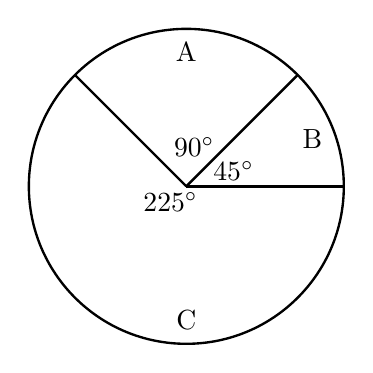
\begin{tikzpicture}
	\draw[line width=0.03cm] (0,0) circle (2);
	\draw[line width=0.03cm] (0,0) -- (2,0);
	\draw[line width=0.03cm] (0,0) -- (1.414,1.414);
	\draw[line width=0.03cm] (0,0) -- (-1.414,1.414);
	\node at (0,-1.7) {C};
	\node at (1.6,0.6) {B};
	\node at (0,1.7) {A};
	\node at (0.6,0.2) {$45^\circ$};
	\node at (0.1,0.5) {$90^\circ$};
	\node at (-0.2,-0.2) {$225^\circ$};
	\end{tikzpicture}
	\] \par
If you spin this wheel, what is the probability that the spinner lands in the region labeled `C'?
	\begin{enumerate}[A.]
	\item $\frac{1}{2}$
	\item $\frac{2}{3}$
	\item $\frac{5}{8}$
	\item $\frac{7}{8}$
	\end{enumerate}

\vfill

% Question 12
\question Below are box plots for the exam scores for students in a Mathematics class, broken down by gender. The women are represented by red and men by blue. 
	\[
	\begin{tikzpicture}
	\begin{axis}[
%	ytick={1,2}
	yticklabels={Men, Women}]
	\addplot+[
	boxplot prepared={
	median=65,
	upper quartile=72,
	lower quartile=63,
	upper whisker=85.5,
	lower whisker=49.5
	},
	line width=0.03cm
	] coordinates {};
	\addplot+[
	boxplot prepared={
	median=80,
	upper quartile=83,
	lower quartile=78,
	upper whisker=90.5,
	lower whisker=70.5
	},
	line width=0.03cm
	] coordinates {};
	\end{axis}
	\end{tikzpicture}
	\]
Which of the following statements is most accurate?
	\begin{enumerate}[A.]
	\item On average, the women did better and the men had more varied scores.
	\item On average, the men did better and the women had more varied scores.
	\item On average, the women did better and the men had less varied scores. 
	\item On average, the men did better and the women had less varied scores. 
	\end{enumerate}

\vfill

% Question 13
\question Let $C$ be the set of cars, $O$ be the set of objects that were made more than five years ago, and $R$ be the set of red objects. Which of the following best describes an element of $(C \cap O^c) \cup (C \cap R)$?
	\begin{enumerate}[A.]
	\item A red car that was made more than 5 years ago.
	\item A red car that was made less than 5 years ago.
	\item A red car or a car made more than 5 years ago.
	\item A red car or a car made less than 5 years ago.
	\end{enumerate}

\vfill

% Question 14
\question How many passwords with 6~characters can be made using the first five letters of the alphabet and the numbers 0--4?
	\begin{enumerate}[A.]
	\item 10
	\item 531,441
	\item 1,000,000
	\item 3,628,800
	\end{enumerate}

\vfill

% Question 15
\question Suppose you give a weekend tour at your college. You ask each of the students how many colleges they have visited and whether they plan to enroll as a part or full time student. The summary of the data you gathered is given below. \par
	\begin{table}[H]
	\centering
	\begin{tabular}{|c|c|c|c|} \hline
	& One College & Two Colleges & Three or More \\ \hline
	Full Time & 3 & 4 & 8 \\ \hline
	Part Time & 5 & 6 & 1 \\ \hline
	\end{tabular}
	\end{table} \par
If you randomly selected a student that was on the tour, what is the probability that they were planning on being full time and had visited more than one college?
	\begin{enumerate}[A.]
	\item $0.148$
	\item $0.296$
	\item $0.444$
	\item $0.800$
	\end{enumerate}

\vfill

% Question 16
\question Which of the following would not be appropriate to use to represent the set of average monthly temperatures from January 2000 to December 2019?
	\begin{enumerate}[A.]
	\item A dot plot.
	\item A bar graph.
	\item A stem-and-leaf plot.
	\item A histogram.
	\end{enumerate}

\vfill

% Question 17
\question Which of the following is the cardinality of the set of even numbers from 10 to 620 (including 0 and 100)?
	\begin{enumerate}[A.]
	\item 290
	\item 305
	\item 306
	\item 610
	\end{enumerate}

\vfill

% Question 18
\question How many six-digit numbers have exactly one seven in their digits?
	\begin{enumerate}[A.]
	\item 7,290
	\item 100,000
	\item 142,857
	\item 321,489
	\end{enumerate}

\vfill

% Question 19
\question Suppose you give a weekend tour at your college. You ask each of the students how many colleges they have visited and whether they plan to enroll as a part or full time student. The summary of the data you gathered is given below. \par
	\begin{table}[H]
	\centering
	\begin{tabular}{|c|c|c|c|} \hline
	& One College & Two Colleges & Three or More \\ \hline
	Full Time & 3 & 4 & 8 \\ \hline
	Part Time & 5 & 6 & 1 \\ \hline
	\end{tabular}
	\end{table}
If you randomly selected a student that was on the tour, assuming they had visited more than one college, what is the approximate probability they planned on being a full time student?
	\begin{enumerate}[A.]
	\item $0.444$
	\item $0.632$
	\item $0.703$
	\item $0.815$
	\end{enumerate}

\vfill

% Question 20
\question Robert calculates that, on average, they make \$47.50 in profit for each person that attends one of the baseball games at the stadium where he works. If there were 8,400 people that attended the last game, approximately how much profit did the stadium make?
	\begin{enumerate}[A.]
	\item \$8,400
	\item \$399,000
	\item \$420,000
	\item \$1,500,000
	\end{enumerate}

\vfill

% Question 21
\question If $A= \{ a, b, a, c, d, e \}$ and $B= \{ a, b, e, e \}$, which of the following is the set $A \cap B$?
	\begin{enumerate}[A.]
	\item $\{ a, a, b \}$
	\item $\{ a, b, e \}$
	\item $\{ a, a, b, d, e, e \}$
	\item None of the above
	\end{enumerate}

\vfill

% Question 22
\question What is the cardinality of the set $A= \{ 1, 1, 2, 2, 3, 3, \ldots, 10, 10 \}$?
	\begin{enumerate}[A.]
	\item 4
	\item 8
	\item 10
	\item 20
	\end{enumerate}

\vfill

% Question 23
\question The chart below summarizes the number of students, broken down by gender, that enjoy Christmas, Thanksgiving, or neither of those two as their favorite holiday. \par
	\begin{table}[H]
	\centering
	\begin{tabular}{|c|c|c|c|} \hline
	& Christmas & Thanksgiving & Neither \\ \hline
	Boy & 6 & 4 & 2 \\ \hline
	Girl & 5 & 3 & 8 \\ \hline
	\end{tabular}
	\end{table} \par
If you select one of these children at random, what is the probability that they liked Thanksgiving best, assuming you selected a boy?
	\begin{enumerate}[A.]
	\item $0.143$
	\item $0.250$
	\item $0.333$
	\item $0.571$
	\end{enumerate}

\vfill

% Question 24
\question Which of the following is not a measure of `averageness' for a set of data?
	\begin{enumerate}[A.]
	\item Mean
	\item Median
	\item Mode
	\item Standard Deviation
	\end{enumerate}

\vfill

% Question 25
\question Let $N$ be the set of numbers from 1 to 30 (including 1 and 30) and $T$ be the set of multiples of 2 or 3. What is $|N - T|$?
	\begin{enumerate}[A.]
	\item 10
	\item 15
	\item 20
	\item 25
	\end{enumerate}

\vfill

% Question 26
\question Charlie is going to invite four friends to go with him on a camping trick. He has seven friends that are interested in the trip. How many possible groups of friends can he invite to go on the trip?
	\begin{enumerate}[A.]
	\item 7
	\item 24
	\item 35
	\item 5,040
	\end{enumerate}

\vfill

% Question 27
\question Peter works with a small research group of 30 people. In the group, there are ten people that work in Mathematics and fifteen that work in Biology with four researchers that work in both areas. What is the probability that if you randomly select on of the researchers that they either work in neither or both Mathematics and Biology.
	\begin{enumerate}[A.]
	\item $\frac{1}{6}$
	\item $\frac{3}{10}$
	\item $\frac{1}{3}$
	\item $\frac{13}{30}$
	\end{enumerate}

\vfill

% Question 28
\question Gloria works at a company whose salaries are normally distributed with mean \$50,000 and standard deviation \$18,000. Approximately percent of works earn more than \$65,000 at the company?
	\begin{enumerate}[A.]
	\item 20.3\%
	\item 68.8\%
	\item 79.7\%
	\item 83.3\%
	\end{enumerate}

\vfill

% Question 29
\question Suppose that $A= [-10, 50)$ and $B= (0, 100)$. Which of the following is $A \cap B$?
	\begin{enumerate}[A.]
	\item $[-10, 100)$
	\item $(0, 50)$
	\item $[0, 50)$
	\item $[0, 50]$
	\end{enumerate}

\vfill

% Question 30
\question Fifteen different businesses are under consideration for an award for `Best Business in Scranton.' The organization responsible for the award will choose one winner and one different team for an honorable mention. How many different choices do they have for these two awards?
	\begin{enumerate}[A.]
	\item 2
	\item 15
	\item 105
	\item 210
	\end{enumerate}



\newpage
\vfill



% Question 31
\question Suppose you roll a die three times. Approximately what is the probability that you roll at least one three?
	\begin{enumerate}[A.]
	\item $0.005$
	\item $0.421$
	\item $0.579$
	\item $0.995$
	\end{enumerate}

\vfill

% Question 32
\question Consider the normal distribution plotted below.
	\[
	\fbox{
	\begin{tikzpicture}[scale=2,every node/.style={scale=0.5}]
	\begin{axis}[
%	grid=both,
	axis lines=middle,
	ticklabel style={fill=blue!5!white},
	axis y line= none,
	xmin= -10.5, xmax=10.5,
	ymin= -0.5, ymax=0.2,
	xtick={-10,-8,...,10},
	ytick={-10,-8,...,10},
	minor x tick num = 1,
	minor y tick num = 1,
	xlabel=\(x\),ylabel=\(y\),
	]
	\addplot[line width=0.03cm,domain=-10:10,samples=100] {gauss(1,3)};
	\end{axis}
	\end{tikzpicture}
	}
	\] 
Which of the following are most likely the mean and standard deviation for this distribution?
	\begin{enumerate}[A.]
	\item $\mu= 1$, $\sigma= 1$
	\item $\mu= 3$, $\sigma= 1$
	\item $\mu= 1$, $\sigma= 3$
	\item $\mu= 6$, $\sigma= 1$
	\end{enumerate}

\vfill

% Question 33
\question Suppose that $A= \{ a, a, b, c, c, d, e, e \}$ and $B= \{ a, b, d, e, f, g, h, a \}$. Which of the following is the cardinality of $A \cup B$?
	\begin{enumerate}[A.]
	\item 8
	\item 12
	\item 13
	\item 16
	\end{enumerate}

\vfill

% Question 34
\question A very large number of orange soda, grape soda, and cherry soda are on a table. You are going to take three sodas to take back to your friends. How many different ways can you choose the three sodas?
	\begin{enumerate}[A.]
	\item 1
	\item 6
	\item 10
	\item 27
	\end{enumerate}

\vfill

% Question 35
\question Suppose that you roll a pair of die. What is the probability that you roll a four and a six?
	\begin{enumerate}[A.]
	\item $\frac{1}{36}$
	\item $\frac{1}{18}$
	\item $\frac{1}{6}$
	\item $\frac{1}{3}$
	\end{enumerate}

\vfill

% Question 36
\question The lengths (in inches) of various leaves was gathered by students working in the field. Their data is given below.
	\[
	1.6 \qquad 2.1 \qquad 1.8 \qquad 2.4 \qquad 1.9 \qquad 2.8 \qquad 2.6 \qquad 1.9 \qquad 2.0 \qquad 2.6
	\] 
Using the median as a measure of center, which of the following possible leaf lengths (in inches) would not represent an outlier given this data.
	\begin{enumerate}[A.]
	\item 0.6
	\item 0.8
	\item 3.5
	\item 3.8
	\end{enumerate}

\vfill

% Question 37
\question Which of the following numbers is an element of the set $S= \{ 3n + 8 \colon n \text{ is an positive integer} \}$?
	\begin{enumerate}[A.]
	\item 2
	\item 8
	\item 20
	\item 25
	\end{enumerate}

\vfill

% Question 38
\question You have six different paintings from two different artists. One artist contributed four paintings while another contributed two. How many different orders can you hang them up on the wall if each artist must have a painting on either the far left or far right in the arrangement?
	\begin{enumerate}[A.]
	\item 48
	\item 192
	\item 384
	\item 720
	\end{enumerate}



\newpage
\vfill



% Question 39
\question You have a bag filled with 12 red marbles and 8 blue marbles. Suppose you reach into the bag, grab a marble, and then set it aside a total of three times. What is the approximate probability that all three marbles were blue?
	\begin{enumerate}[A.]
	\item $0.042$
	\item $0.049$
	\item $0.064$
	\item $0.40$
	\end{enumerate}

\vfill

% Question 40
\question Jose has been gathering data on the amount of snowfall in his local community. He reads off the snow levels using a ruler attached to a wall outside his classroom. He finds the mean and standard deviation for the data he gathered. However, after performing this computation, he realizes that the ruler was 0.2" above the ground. If Jose corrects this error in his data, what will happen to the mean and standard deviation for his data?
	\begin{enumerate}[A.]
	\item The mean and standard deviation will decrease.
	\item The mean will decrease, but the standard deviation will stay the same.
	\item The mean will decrease, but the standard deviation will increase.
	\item The mean will stay the same, but the standard deviation will decrease. 
	\end{enumerate}

\vfill

% Question 41
\question Let $P$ be the set of all prime numbers and $O$ be the set of all odd numbers. Which of the following is true?
	\begin{enumerate}[A.]
	\item $P \subseteq O$
	\item $O \subseteq P$
	\item $P= O$
	\item $P \neq O$
	\end{enumerate}

\vfill

% Question 42
\question How many different arrangements are there using the letters of the word `field' if the arrangement must start and end with a vowel?
	\begin{enumerate}[A.]
	\item 6
	\item 12
	\item 60
	\item 120
	\end{enumerate}



\newpage
\vfill



% Question 43
\question You interview 25 children about whether they like swimming or riding their bike. Of these children, two say they only enjoy swimming, five say they only enjoy biking, and ten say they do not enjoy swimming nor biking. If you select a child that you interviewed at random, what is the probability that they enjoyed swimming or biking?
	\begin{enumerate}[A.]
	\item $0.28$
	\item $0.40$
	\item $0.60$
	\item $0.68$
	\end{enumerate}

\vfill

% Question 44
\question Consider the data values given below.
	\[
	0 \qquad 20 \qquad 10 \qquad 50 \qquad 40 \qquad 10
	\]
Which of the following is the correct ordering for this data?
	\begin{enumerate}[A.]
	\item mode $<$ median $<$ mean
	\item median $<$ mean $<$ mode
	\item mean $<$ median $<$ mode
	\item mode $<$ mean $<$ median
	\end{enumerate}

\vfill

% Question 45
\question Let $H$ be event that a randomly selected person in the United States has bought a home. Let $Y$ be the event that a randomly selected person in the United States is under 30 years old. Which of the following is most correct?
	\begin{enumerate}[A.]
	\item The events $H$ and $Y$ are mutually exclusive but not independent. 
	\item The events $H$ and $Y$ are mutually exclusive and independent. 
	\item The events $H$ and $Y$ are not mutually exclusive and not independent. 
	\item The events $H$ and $Y$ are not mutually exclusive but are independent. 
	\end{enumerate}

\vfill

% Question 46
\question Consider the data given below.
	\[
	8 \qquad 9 \qquad 10 \qquad 11 \qquad 11 \qquad 11 \qquad 12 \qquad 14 \qquad 19
	\]
Which of the following is the 5-number summary for this dataset?
	\begin{enumerate}[A.]
	\item 8, 9, 11, 14, 19
	\item 8, 9.5, 11, 13, 19
	\item 8, 10, 11, 12, 19
	\item 8, 10.5, 11, 11.5, 19
	\end{enumerate}

\vfill

% Question 47
\question The chart below summarizes the number of students, broken down by gender, that enjoy Christmas, Thanksgiving, or neither of those two as their favorite holiday. \par
	\begin{table}[H]
	\centering
	\begin{tabular}{|c|c|c|c|} \hline
	& Christmas & Thanksgiving & Neither \\ \hline
	Boy & 6 & 4 & 2 \\ \hline
	Girl & 5 & 3 & 8 \\ \hline
	\end{tabular}
	\end{table} \par
If you select one of these children at random, what is the approximate probability that they are a girl or their favorite holiday is Thanksgiving?
	\begin{enumerate}[A.]
	\item $0.107$
	\item $0.607$
	\item $0.714$
	\item $0.857$
	\end{enumerate}

\vfill

% Question 48
\question Consider the box and whisker for a set of data that is given below.
	\[
	\begin{tikzpicture}[scale=0.85]
	\begin{axis}[
%	ytick={1,2}
	xmin=30, xmax=100, 
	xtick={30,40,...,100},
	ytick={},
	yticklabels={}
	]
	\addplot+[
	boxplot prepared={
	median=72,
	upper quartile=85,
	lower quartile=62,
	upper whisker=91,
	lower whisker=45
	},line width=0.03cm
	] coordinates {};
	\end{axis}
	\end{tikzpicture}
	\]
Which of the following is most likely the median and IQR for this dataset?
	\begin{enumerate}[A.]
	\item median$=$ 72, IQR$=$ 23 
	\item median$=$ 72, IQR$=$ 12
	\item median$=$ 75, IQR$=$ 23
	\item median$=$ 75, IQR$=$ 12
	\end{enumerate}

\vfill

% Question 49
\question If $A$ and $B$ are subsets of the same set, which of the following must be the same as $A - B$?
	\begin{enumerate}[A.]
	\item $A \cap B^c$
	\item $(A \cap B)^c$
	\item $A \cap B$
	\item $A^c \cup B^c$
	\end{enumerate}

\vfill

% Question 50
\question If $A$ is an event that occurs with probability 0.20 and $B$ is an event that occurs with probability 0.35. Which of the following is not a possible value for the probability that $A$ and $B$ both occur?
	\begin{enumerate}[A.]
	\item 0.10
	\item 0.20
	\item 0.60
	\item Cannot be determined with the given information.
	\end{enumerate}

\end{questions}
\end{document}